\documentclass{article}

\usepackage[english]{babel}
\usepackage[utf8x]{inputenc}
\usepackage{amsmath}
\usepackage{amssymb}
\usepackage{amsthm}
\usepackage{graphicx}
\usepackage{hyperref}
\usepackage[colorinlistoftodos]{todonotes}
\setlength\parindent{0pt}

\begin{document}

\section*{Question 3}
The MATLAB code is in Q3/code folder, with myMainScript.m being the main file. PerformOMP is the backbone which implements the OMP algorithm. The code to combine overlapping patches to generate an image has been borrowed from \href{http://spams-devel.gforge.inria.fr/}{SPAMS toolbox}. The files with prefix mexCombine are used and are copied as is.

Note: The code takes approximately 15 minutes to run.

The plots are stored in Q3/results as image files. The error values are in Q3/data/mse.txt with values written in decreasing order of f (equivalently, more fewer measurements) taken.\\

\begin{figure}[!h]
    \centering
    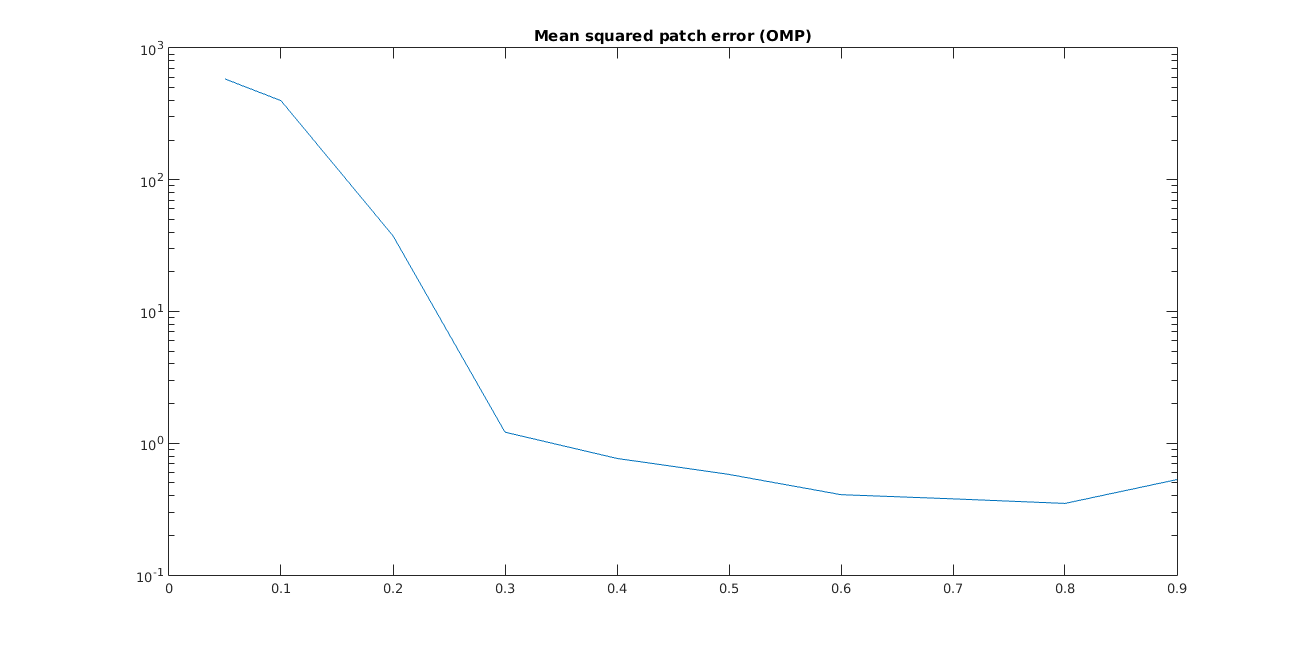
\includegraphics[width=0.8\textwidth]{mspe_omp}
    \caption{Mean squared patch error (OMP). x-axis is f and y axis is error values (log scale)}
\end{figure}

\begin{figure}[!h]
    \centering
    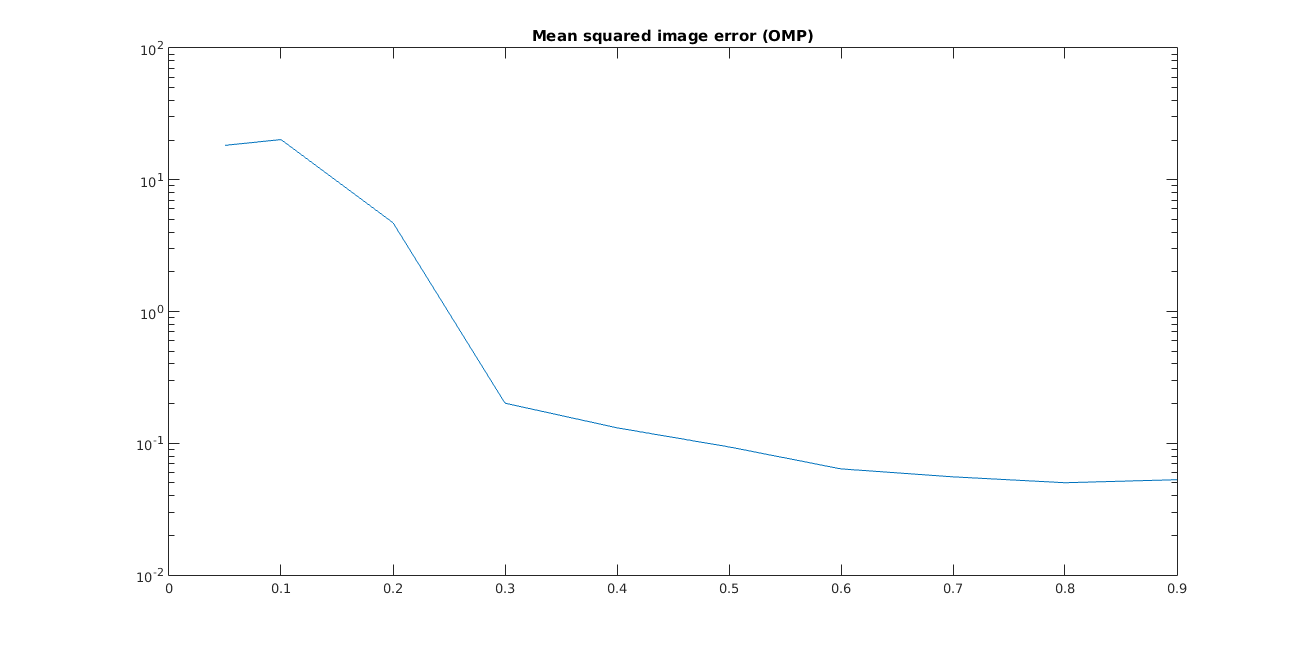
\includegraphics[width=0.8\textwidth]{msie_omp}
    \caption{Mean squared image error (OMP). x-axis is f and y axis is error values (log scale)}
\end{figure}

\begin{figure}[!h]
    \centering
    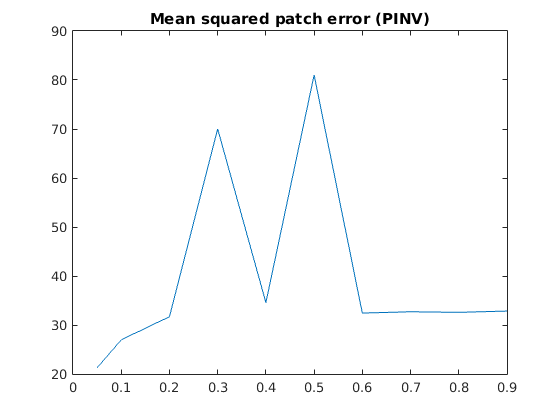
\includegraphics[width=0.8\textwidth]{mspe_pinv}
    \caption{Mean squared patch error (PINV). x-axis is f and y axis is error values}
\end{figure}

\begin{figure}[!h]
    \centering
    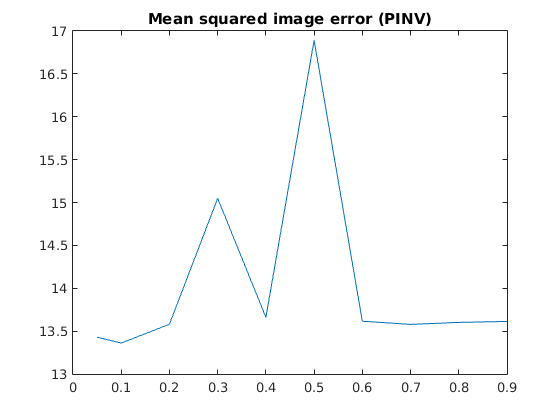
\includegraphics[width=0.8\textwidth]{msie_pinv}
    \caption{Mean squared image error (PINV). x-axis is f and y axis is error values}
\end{figure}


\subsection*{Observations}
\begin{enumerate}
    \item In OMP, the mean squared errors are low till f = 0.3. For even lesser data, the error shoots up very rapidly.
    \item In simple pseudo-inverse, even a small amount of compression degrades the reconstruction. No related in accuracy with f can be observed.
    \item In both the cases, the mean squared error over images are less than that over patches. This may be due to the fact that the value for a pixel in the image is calculated by averaging over multiple patches. This reduces the effect of Gaussian noise.
\end{enumerate}



\end{document}